\chapter{Evaluation}
\label{ch:evaluation}
This chapter will cover the execution and evaluation of our benchmark with the workloads specified in section~\ref{ch:design:se:workloads}.
We will present the results of each workload and have a discussion on them directly after that.

A conclusion will be drawn in section~\ref{ch:futureWork:se:conclusion} in the next chapter.

\section{Objective}
The main goal is to see,
if the databases are capable of handling the production workloads.
Besides that we will investigate if we can generalise graph database benchmark results by comparing our results with the results of other studies examining the performance of graph databases with social network graphs.
The generalisation would allow to use benchmark results created with social network graphs for the evaluation of performance of graph databases in an industrial environment.

We will measure the time per operation and with the average we can calculate the throughput in $ \frac{operations}{s} $,
that way we can compare the databases without take into account the overhead of the benchmark itself,
which would be reflected in the overall run time.

In section~\ref{ch:evaluation:se:overview} we will show which workloads we will compare with each other.

\section{Setup}
In this section we will describe the software and hardware we used to execute the benchmark.

\subsection{Hardware}
The machine used for the benchmark had the specifications shown in table~\ref{tab:hardware}.

\begin{table}[!h]
  \begin{minipage}{\textwidth}
    \begin{tabularx}{\textwidth}{ | l | X | }
      \hline
      Component & Description \\ \hline \hline
      CPU & Intel i7-3770K @ 3.5GHz \\ \hline
      RAM & 16GB DDR3 @ 1.600MHz \\ \hline
      Storage & Seagate ST2000DL003 2 TB 5900rpm, only a 400GB partition was used \\ \hline
      GPU & NVIDIA GeForce GTX 670 \\ \hline
    \end{tabularx}
  \end{minipage}
  \caption{The hardware specifications of the machine used for the benchmark.}
  \label{tab:hardware}
\end{table}

\subsection{Software}
The versions of the software components we used are shown in table~\ref{tab:software}.

\begin{table}[!h]
  \begin{minipage}{\textwidth}
    \begin{tabularx}{\textwidth}{ | X | X | }
      \hline
      Software & Version \\ \hline \hline
      Ubuntu & 17.10 \\ \hline
      Java & 1.8.0\_171 \\ \hline
      OpenSSH & 7.5p1 \\ \hline
      YCSB & 0.14.0-SNAPSHOT \\ \hline
      ApacheJena & 3.6.0 \\ \hline
      Neo4j & 3.3.4 \\ \hline
      OrientDB & 2.2.33 \\ \hline
      Sparksee & 5.2.3 \\ \hline
    \end{tabularx}
  \end{minipage}
  \caption{The software specifications of the machine used for the benchmark.}
  \label{tab:software}
\end{table}

\section{Overview}
\label{ch:evaluation:se:overview}
In figure~\ref{fig:executionWorkflow} the execution process is illustrated and explained in the following enumeration.

\begin{enumerate}[label=Step \arabic*:,widest=Step 1,leftmargin=*]
  \item One workload is chosen from the set of workloads.
  \item The dataset is created for that workload.
  \item One database is chosen from the set of databases.
  \item The workload is executed on the database with the created dataset.
  \item The results of the benchmark run are stored in a folder specific to the constellation of workload,
  database and execution pass.
  \item Repeat from Step 4 three times.
  \item Repeat from Step 3 until all databases ware benchmarked.
  \item Repeat from Step 1 until all workloads have been executed.
\end{enumerate}

\begin{figure}[!h]
  \includegraphics[width=\textwidth]{images/executionWorkflow}
  \caption{Workflow for the execution process.}
  \label{fig:executionWorkflow}
\end{figure}

In table~\ref{tab:throughputOverview} and~\ref{tab:productionOverview} the groups of workloads we are comparing with each other are shown.
The naming of the workloads is similar to the naming introduced in section~\ref{ch:design:se:workloads}.

\begin{table}
  \begin{minipage}{\textwidth}
    \centering
    \begin{tabularx}{\textwidth}{ | l | l | l | X | }
      \hline
      Section & First workload & Other workload(s) & Units of measurement \\ \hline
      \ref{ch:evaluation:se:probingNodeCount} & 1. With Index & 2.-5. With Index & Inserts/second, total time, database size \\ \hline
      \ref{ch:evaluation:se:probingNodeCount} & 1. Without Index & 2.-5. Without Index & Inserts/second \\ \hline
      \ref{ch:evaluation:se:probingNodeCount} & n.\footnote{the workload with the largest possible number of nodes in terms of execution time} With Index & n. Without Index & Inserts/second \\ \hline
      \ref{ch:evaluation:se:probingNodeSize} & 1. Node Size & 2.-5. Node Size & Inserts/second, database size \\ \hline
      \ref{ch:evaluation:se:differenceEdges} & 1. No Edges & 2. No Edges & Inserts/second \\ \hline
      \ref{ch:evaluation:se:differenceEdges} & n. With Index & 1. No Edges & Inserts/second \\ \hline
    \end{tabularx}
  \end{minipage}
  \caption{Overview for the throughput workloads. \todo{remove reason and mention in evaluation}}
  \label{tab:throughputOverview}
\end{table}
\begin{table}
  \begin{minipage}{\textwidth}
    \centering
    \begin{tabularx}{\textwidth}{ | l | l | X | X | }
      \hline
      Section & First workload & Other workload(s) & Units of measurement \\ \hline
      \ref{ch:evaluation:se:productComplexity} & 1. Structure & 2.-3. Structure & Inserts/second \\ \hline
      \ref{ch:evaluation:se:productionSuitability} & x.\footnote{every workload will be evaluated} Suitability & - & Total time \\ \hline
      \ref{ch:evaluation:se:retrievingUnderLoad} & 1. Reading & 2. Reading & Reads/second \\ \hline
      \ref{ch:evaluation:se:retrievingUnderLoad} & 1. Scanning & 2. Scanning & Scans/second \\ \hline
      \ref{ch:evaluation:se:retrievingUnderLoad} & 1. Structure & 1. Reading \& 1. Scanning & Operations/second \\ \hline
    \end{tabularx}
  \end{minipage}
  \caption{Overview for the production and retrieval workloads.}
  \label{tab:productionOverview}
\end{table}

After execution we have to combine the results for further inspection.
Figure~\ref{fig:evaluationWorkflow} illustrates this process of evaluation.
With all the results in one place we filtered the measurements for those we wanted,
then we calculated the average over the three benchmark runs we did with every database and workload.
Next,
we grouped the measurements as shown in tables~\ref{tab:throughputOverview} and~\ref{tab:productionOverview}.
And finally,
we create the diagrams shown in subsections "Results" of the following sections and interpret them to draw a conclusion,
which is presented in the "Discussion" subsections.

\begin{figure}[!h]
  \includegraphics[width=\textwidth]{images/evaluationProcess}
  \caption{Workflow of the evaluation process.}
  \label{fig:evaluationWorkflow}
\end{figure}

\section{Throughput}
\label{ch:evaluation:se:throughput}
In this section we will examine the combinations of workloads mentioned in table~\ref{tab:throughputOverview}.
The throughput will show us how well suited the graph databases are in general for applications heavily using insert operations.

Note that in order to insert an edge the start and end node has to be looked up.

\subsection{Probing Node Count}
\label{ch:evaluation:se:probingNodeCount}
Here we will compare how the throughput,
measured in inserts per second,
of the databases is effected by increasing the number of nodes we are inserting into it.
We will also look at the execution time,
to determine a reasonable large dataset in terms of execution time for the upcoming benchmark runs.

The throughput is listed in inserts per seconds,
which include both inserting nodes and inserting edges.

Apache Jena has no option to turn off indexing as mentioned in section~\ref{ch:background:se:apacheJena},
but it is still shown in the diagrams as reference.

\subsubsection{Results}
The first figure~\ref{fig:withIndexThroughput} shows how the different databases perform with an increasing dataset size.
Apache Jena and Neo4j only have values for 1.000 and 10.000 nodes,
because execution with more than 10.000 nodes would take too much time.
Sparksee only delivered results up to 100.000 nodes,
because the free license only included database sizes of up to 1.000.000 elements and a workload with 1.000.000 nodes would contain 2.333.333 elements in total with the edges.

In figure~\ref{fig:withIndexExecutionTime} we see the execution time of the different databases.
At 10.000 nodes Apache Jena and Neo4j took almost an hour for one run,
because of that we did not run it with 100.000 nodes or more.

Table~\ref{tab:withIndexThroughput},
\ref{tab:withIndexExecutionTime} and~\ref{tab:withoutIndexThroughput} show the measured numbers from the figures~\ref{fig:withIndexThroughput},
\ref{fig:withIndexExecutionTime} and~\ref{fig:withoutIndexThroughput} respectively.

\begin{table}[h!]
  \begin{minipage}{\textwidth}
    \centering
    \begin{tabularx}{\textwidth}{ | l | X | X | X | X | X | }
      \hline
      Database/\# Nodes & 1000 & 10000 & 100000 & 1000000 & 10000000 \\ \hline
      apachejena & 8,86 & 7,21 & T & T & T \\ \hline
      neo4j & 11,50 & 8,75 & T & T & T \\ \hline
      orientdb & 884,1 & 2317,07 & 5672,69 & 10112,36 & 8572,34 \\ \hline
      sparksee & 15109,17 & 17829,1 & 16425 & L & L \\ \hline
    \end{tabularx}
  \end{minipage}
  \caption{Throughput in inserts/s rounded to two decimal places of the workload using an index for the different dataset sizes. T indicates that too much time would be needed; L indicated license issues.}
  \label{tab:withIndexThroughput}
\end{table}

\begin{table}[h!]
  \begin{minipage}{\textwidth}
    \centering
    \begin{tabularx}{\textwidth}{ | l | X | X | X | X | X | }
      \hline
      Database/\# Nodes & 1000 & 10000 & 100000 & 1000000 & 10000000 \\ \hline
      apachejena & 263 & 3238 & T & T & T \\ \hline
      neo4j & 203 & 2667 & T & T & T \\ \hline
      orientdb & 3,64 & 10 & 41 & 231 & 2722 \\ \hline
      sparksee & 0,15 & 1,31 & 14 & L & L \\ \hline
    \end{tabularx}
  \end{minipage}
  \caption{Execution time in seconds of the workload using an index for the different dataset sizes. T indicates that too much time would be needed; L indicated license issues.}
  \label{tab:withIndexExecutionTime}
\end{table}

\begin{table}[h!]
  \begin{minipage}{\textwidth}
    \centering
    \begin{tabularx}{\textwidth}{ | l | X | X | X | X | X | }
      \hline
      Database/\# Nodes & 1000 & 10000 & 100000 & 1000000 & 10000000 \\ \hline
      apachejena & 8,79 & 7,41 & T & T & T \\ \hline
      neo4j & 12,3 & 8,83 & T & T & T \\ \hline
      orientdb & 1020,81 & 2357,49 & 4616,85 & 9395,86 & 8415,18 \\ \hline
      sparksee & 4715,63 & 635,17 & 63,37 & L & L \\ \hline
    \end{tabularx}
  \end{minipage}
  \caption{Throughput in inserts/s rounded to two decimal places of the workload using no index for the different dataset sizes. T indicates that too much time would be needed; L indicated license issues.}
  \label{tab:withoutIndexThroughput}
\end{table}

\begin{figure}[h!]
  \centering
  \includegraphics[width=.75\textwidth]{images/throughput/withIndexThroughput}
  \caption{This figure shows the throughput in inserts/second of every database over different dataset sizes.}
  \label{fig:withIndexThroughput}
\end{figure}

\begin{figure}[h!]
  \centering
  \includegraphics[width=.75\textwidth]{images/throughput/withIndexExecutionTime}
  \caption{The execution time of the databases is shown over different dataset sizes.}
  \label{fig:withIndexExecutionTime}
\end{figure}

Figure~\ref{fig:withoutIndexThroughput} shows the throughput over different dataset sizes without using an index.
In figure~\ref{fig:withWithoutIndexThroughputFixNodes} we see a comparison of using an index and not with a dataset size of 10.000 nodes.

\begin{figure}[h!]
  \centering
  \includegraphics[width=.75\textwidth]{images/throughput/withoutIndexThroughput}
  \caption{This diagram shows the throughput in inserts per second while using no index.}
  \label{fig:withoutIndexThroughput}
\end{figure}

\begin{figure}[h!]
  \centering
  \includegraphics[width=.75\textwidth]{images/throughput/withWithoutIndexThroughputFixNodes}
  \caption{The throughput at a fixed dataset size to compare between indexing and not.}
  \label{fig:withWithoutIndexThroughputFixNodes}
\end{figure}

\subsubsection{Discussion}
Figure~\ref{fig:withWithoutIndexThroughputFixNodes} shows us,
that there is no performance change for Jena, Neo4j and OrientDB in using an index or not.
Sparksee shows a significant drop in throughput without the use of an index.
That is what we expected,
because the throughput also contains insertions of edges,
which have to look up nodes,
what is faster with an index.
For the other databases the lack of difference in performance might by,
that the benefit of using an index to retrieve the nodes for an edge is equalised by the time they take to insert the nodes into the index.

The execution time grows linearly,
which is a good sign,
because that means that the databases do scale for larger amounts of data.

If we compare the archived throughput with our target throughput of $ 11743,67 \frac{inserts}{s} $,
we see that Sparksee exceeds our target with $ 16435 \frac{inserts}{s} $.
OrientDB misses our goal slightly,
at the larges dataset it only archived a throughput of $ 8572 \frac{inserts}{s} $.
Jena and Neo4j didn't even reach $ 10 \frac{inserts}{s} $.
These throughput values are measured with another data structure and node size than the one we will use for the suitability workload,
so we will investigate the factors differentiating this workload from the suitability workload and reference these results again in section~\ref{ch:evaluation:se:suitabilityDiscussion}.

From these results alone,
without looking at read performance separately we can say,
that an index is useful,
even for insert operations,
because edges need to look up two nodes,
which is faster when an index is used.

\subsection{Probing Node Size}
\label{ch:evaluation:se:probingNodeSize}
In this subsection we will take a look at how the databases perform with different node property sizes.
We will pick a dataset size of 10.000 nodes,
as all database have a reasonable execution time with that amount of nodes.

By investigating the performance under node size variation,
we will see if the databases can store larger number of data in one node.
That can be useful depending on the use case,
in our example given by the industry only a two-digit number is stored,
but it could be desirable to store longer number or more complex information.

\subsubsection{Results}
In figure~\ref{fig:nodeSize} we see,
how an increasing node size has an impact on insert throughput.

Sparksee only has values for node sizes up to $ 1KB $,
because the property we used to store the value of the node only supports up to 2048 characters or Bytes.

Figure~\ref{fig:sizeDatabaseSize} shows the size of the database folder,
in which the database stores its files.

Table~\ref{tab:nodeSize} and~\ref{tab:sizeDatabaseSize} show the numbers used for the figures~\ref{fig:nodeSize} and~\ref{fig:sizeDatabaseSize} respectively.

\begin{table}[h!]
  \begin{minipage}{\textwidth}
    \centering
    \begin{tabularx}{\textwidth}{ | X | X | X | X | X | X | X | }
      \hline
      Node Size (Byte)/ \newline
      Database & 10 & 100 & 1000 & 10000 & 100000 & 1000000 \\ \hline
      apachejena & 7,21 & 9,66 & 7,83 & 7,54 & 6,21 & 4,92 \\ \hline
      neo4j & 8,75 & 11,47 & 8,31 & 8,59 & 8,17 & 4,06 \\ \hline
      orientdb & 2317,07 & 2521,90 & 3141,73 & 1976,84 & 487,21 & 14,10 \\ \hline
      sparksee & 17829,10 & 17155,63 & 15670,67 & x & x & x \\ \hline
    \end{tabularx}
  \end{minipage}
  \caption{Throughput in inserts/s rounded to two decimal places of the workload using different node sizes. x indicates issues with storing large values.}
  \label{tab:nodeSize}
\end{table}

\begin{table}[h!]
  \begin{minipage}{\textwidth}
    \centering
    \begin{tabularx}{\textwidth}{ | X | X | X | X | X | X | X | }
      \hline
      Node Size (Byte)/ \newline
      Database & 10 & 100 & 1000 & 10000 & 100000 & 1000000 \\ \hline
      apachejena & 15 & 16 & 25 & 113 & 994 & 9600 \\ \hline
      neo4j & 24 & 29 & 49 & 244 & 2200 & 22000 \\ \hline
      orientdb & 75 & 77 & 98 & 172 & 1300 & 9500 \\ \hline
      sparksee & 4,7 & 6 & 15 & x & x & x \\ \hline
    \end{tabularx}
  \end{minipage}
  \caption{Database sizes of the workload using different node sizes. x indicates issues with storing large values.}
  \label{tab:sizeDatabaseSize}
\end{table}

\begin{figure}[h!]
  \centering
  \includegraphics[width=.75\textwidth]{images/throughput/nodeSize}
  \caption{Insert throughput over different node sizes with 10.000 nodes total.}
  \label{fig:nodeSize}
\end{figure}

\begin{figure}[h!]
  \centering
  \includegraphics[width=.75\textwidth]{images/throughput/sizeDatabaseSize}
  \caption{The size of the databases over growing node sizes.}
  \label{fig:sizeDatabaseSize}
\end{figure}

\subsubsection{Discussion}
Figure~\ref{fig:nodeSize} show that the throughput of Jena and Neo4j is quite low and it doesn't show much difference with larger node sizes,
but at $ 1MB $ we can see that the performance decreases even more.

For OrientDB we see good performance up to $ 1KB $,
it starts to decline for node sizes of $ 10KB $ and above with a significant drop at $ 1MB $.

Sparksee has the highest throughput of all four databases,
but as it could only handle sized of up to $ 2KB $ or $ 1KB $ in our test scenario.
In that range the other databases also show no noteworthy change in performance,
so we can't draw a conclusion about the behaviour of Sparksee with larger node sizes.

In figure~\ref{fig:sizeDatabaseSize} we see that the database size grows linearly with the node size,
from $ 10KB $ and above.
So,
for smaller node values the overhead of the database itself determines the size of the database.

When we look closely at the values of Neo4j,
we can see that they are above the other databases.
In fact,
at $ 1MB $ node size,
which would result in $ 10GB $ data for 10.000 nodes,
Neo4js database folder had a size of $ 22GB $,
so the overhead is more than the data itself.

\subsection{Difference without Edges}
\label{ch:evaluation:se:differenceEdges}
Here we will investigate how the absents of edges has an impact on performance.
These workloads to not represent a real-world scenario,
but they will provide us knowledge about how much inserting nodes costs compared to edges,
as for every edge its start and end node have to be looked up.

Apache Jena always uses an index,
but it is still shown in both parts of the diagram as reference.

\subsubsection{Results}
Figure~\ref{fig:noEdges} shows us the difference in using an index compared to not doing so,
while only inserting nodes.
Table~\ref{tab:noEdges} shows the measured values for this workload.

\begin{table}[h!]
  \begin{minipage}{\textwidth}
    \centering
    \begin{tabular}{ | l | l | l | }
      \hline
      Database & Index & No Index \\ \hline
      apachejena & 9,95 & 9,72 \\ \hline
      neo4j & 6,66 & 12,27 \\ \hline
      orientdb & 1425,64 & 1488,03 \\ \hline
      sparksee & 19592,96 & 20316,55 \\ \hline
    \end{tabular}
  \end{minipage}
  \caption{Throughput in inserts/s rounded to two decimal places of the workload comparing inserts without edges with and without an index.}
  \label{tab:noEdges}
\end{table}

\begin{figure}[h!]
  \centering
  \includegraphics[width=.75\textwidth]{images/throughput/noEdges}
  \caption{Difference between using an index and not while using no edges.}
  \label{fig:noEdges}
\end{figure}

In figure~\ref{fig:indexNoEdges10000Nodes} we see a comparison of all databases between using edges and not with a dataset size of 10.000 nodes.

\begin{figure}[h!]
  \centering
  \includegraphics[width=.75\textwidth]{images/throughput/indexNoEdges10000Nodes}
  \caption{Comparison of insert throughput between using edges and not.}
  \label{fig:indexNoEdges10000Nodes}
\end{figure}

\subsubsection{Discussion}
\todo{Do edges effect throughput}
As expected in figure~\ref{fig:noEdges} we can see,
that using an index does not benefit the insert performance for nodes.
Only Neo4j shows a notable difference for the node insert throughput with the use of an index the throughput drop to $ 6,6 \frac{inserts}{s} $ from $ 12 \frac{inserts}{s} $ without an index.

Figure~\ref{fig:indexNoEdges10000Nodes} shows,
that the insert throughput of Apache Jena is slightly lower when using edges.

\section{Production Simulation}
\label{ch:evaluation:se:productionSimulation}
The workload results presented in this section will cover the production specific variables.
The first one being product complexity and the other one execution time.

\subsection{Product Complexity}
\label{ch:evaluation:se:productComplexity}
\note{Structure has no effect, how the edges are connected between the nodes. But edges count matters as we see in comparison to the other benchmarks}
\todo{From Design: Number of edges could effect the throughput, because of inserts. social networks have much more edges to it than our structure}
If the throughput is not effected by using no edges compared to using edges,
we could see,
that for a graph database the structure of the data has no impact on performance.
This result is quite important,
as it would lead to the conclusion,
that we can use the results of other graph database benchmarks for our industrial use case.

The product complexity describes,
how much the tree representing our data structure is widened at three different levels shown in section~\ref{ch:design:se:dataStructure}.

The wider the data structure becomes the less edges we have per node.
That can be interesting if we want to compare the generalisation of the throughput with different graph structures,
which we need to determine if the throughput archived in section~\ref{ch:evaluation:se:probingNodeCount} can be used to draw conclusions about the suitability for the industrial environment.

\subsubsection{Results}
In figure~\ref{fig:structure} and table~\ref{tab:structure} we see the impact a different data structure has on the insert throughput.
"Simple" refers to the structure variables (x, y, z) set to (1, 1, 1),
"More Complex" represents (16, 32, 32) and "Most Complex" (64, 128, 128).

\begin{table}[h!]
  \begin{minipage}{\textwidth}
    \centering
    \begin{tabularx}{\textwidth}{ | l | X | X | X | }
      \hline
      Database & Simple & More Complex & Most Complex \\ \hline
      apachejena & 9,42 & 8,01 & 7,58 \\ \hline
      neo4j & 11,44 & 11,64 & 8,5 \\ \hline
      orientdb & 2606,5 & 2330,12 & 2118,38 \\ \hline
      sparksee & 17345,38 & 17463,8 & 17576,06 \\ \hline
    \end{tabularx}
  \end{minipage}
  \caption{Throughput in inserts/s rounded to two decimal places of the workload comparing different structure parameters.}
  \label{tab:structure}
\end{table}

\begin{figure}[h!]
  \centering
  \includegraphics[width=.75\textwidth]{images/production/structure}
  \caption{Shows the difference in insert throughput over changing data structure.}
  \label{fig:structure}
\end{figure}

\subsubsection{Discussion}
As we see in figure~\ref{fig:structure} the structure of the data as we modelled it,
doesn't effect the throughput of the databases.

For the "simple" workload the have an edge to node ratio of around $ 1.33 $ which is dropping to $ ~1 $ for the "most complex" workload.
Together with the results from~\ref{ch:evaluation:se:differenceEdges} we can say,
that the use of edges has almost no impact on performance and the edge to node ratio also doesn't.

 draw a conclusion about the comparability with other related work using social network graphs,
which have a much higher edge to node ratio,
in order to do so we would have to investigate higher edge to node ratios.

\subsection{Production Suitability}
\label{ch:evaluation:se:productionSuitability}
The production simulations will finally show,
if the databases we chose are capable of storing the necessary amount of data in a specified time interval.

In the discussion of this section we will also investigate the throughput based on the previous workloads.

\subsubsection{Results}
Figure~\ref{fig:singleSuitability} and table~\ref{tab:singleSuitability} show how long OrientDB took,
to store three minutes of production data (1.056.833 nodes).
Sparksee is mentioned with a theoretical time,
since it only allowed us to store 500.000 elements.
We took the throughput during inserting these 500.000 elements and calculated the time it would need to complete the whole workload.

Only OrientDB and Sparksee were used in these workloads,
because Apache Jena and Neo4j would take too long to insert that number of nodes.

\begin{table}[h!]
  \begin{minipage}{\textwidth}
    \centering
    \begin{tabular}{ | l | l | }
      \hline
      Database & Time (s) \\ \hline
      orientdb & 263 \\ \hline
      sparksee & (134) \\ \hline
    \end{tabular}
  \end{minipage}
  \caption{Time needed to execute three minutes of simulated production.
  The value in parentheses indicates a theoretical value,
  which was calculated with the throughput reached until the license ran out of size.}
  \label{tab:singleSuitability}
\end{table}

\begin{figure}[h!]
  \centering
  \includegraphics[width=.75\textwidth]{images/production/singleSuitability}
  \caption{Shows the execution time with a dataset that represents three minutes of production.}
  \label{fig:singleSuitability}
\end{figure}

\subsubsection{Discussion}
\label{ch:evaluation:se:suitabilityDiscussion}
We only executed three minutes of production simulation,
because the throughput of OrientDB does not grow anymore above 1000000 nodes the one-hour workload would not succeed either.

Figure~\ref{fig:singleSuitability} shows us,
that OrientDB did not manage to store three minutes of production simulation in the specified time.

Sparksee could theoretically store that amount without exceeding the time limit,
but since the free license did not allow for the amount of data we used the average util the limit was reached.
Of course,
it could be that the throughput of Sparksee drops with an increasing number of elements in the database,
but we couldn't investigate that.

The difference of this workload compared to the first workload we discussed in section~\ref{ch:evaluation:se:probingNodeCount} is the structure and the node size.
The results of~\ref{ch:evaluation:se:probingNodeSize} and~\ref{ch:evaluation:se:productComplexity} show,
that the structure has no impact on the throughput and the node size has no impact below $ 10KB $,
since we used $ 50B $ we can compare the first measured throughput.

By doing so we see that Sparksee,
again theoretically,
reaches our target throughput of $ 11743 \frac{inserts}{s} $.
OrientDB misses it with only $ 8572 \frac{inserts}{s} $.
These results support our findings for the impact of structure and node size,
as this workload measuring the time correlates with the numbers from the first workload.

\section{Retrieving under load}
\label{ch:evaluation:se:retrievingUnderLoad}
\todo{compare to results of other studies}
This section will cover the results about retrieving data while the database is under load.
First,
we will take a look at how using an index is effecting the read and scan throughput,
then we will compare the throughput of the different operations~(\ref{fig:operationReadScan}) and their impact on the insert operation~(\ref{fig:insertWithWithoutReadScan}).

\subsection{Results}
In figure~\ref{fig:readThroughput10000Nodes},
~\ref{fig:scanThroughput10000Nodes} and table~\ref{tab:readThroughput10000Nodes},
~\ref{tab:scanThroughput10000Nodes} we see the throughput of read and scan operations while using an index and not.

\begin{table}[h!]
  \begin{minipage}{\textwidth}
    \centering
    \begin{tabular}{ | l | l | l | }
      \hline
      Database & Index & No Index \\ \hline
      apachejena & 47 & 49,11 \\ \hline
      neo4j & 954,77 & 795,94 \\ \hline
      orientdb & 8484,44 & 7816,22 \\ \hline
      sparksee & 12411,84 & 989,3 \\ \hline
    \end{tabular}
  \end{minipage}
  \caption{Throughput in reads/s of read operations rounded to two decimal places of the workload using a mix of read and write operations.}
  \label{tab:readThroughput10000Nodes}
\end{table}

\begin{table}[h!]
  \begin{minipage}{\textwidth}
    \centering
    \begin{tabular}{ | l | l | l | }
      \hline
      Database & Index & No Index \\ \hline
      apachejena & 43,58 & 42,56 \\ \hline
      neo4j & 574,17 & 495,58 \\ \hline
      orientdb & 308,93 & 319,89 \\ \hline
      sparksee & 174,28 & 135,41 \\ \hline
    \end{tabular}
  \end{minipage}
  \caption{Throughput in scans/s of scan operations rounded to two decimal places of the workload using a mix of scan and write operations.}
  \label{tab:scanThroughput10000Nodes}
\end{table}

\begin{figure}[h!]
  \centering
  \includegraphics[width=.75\textwidth]{images/responsiveness/readThroughput10000Nodes}
  \caption{Shows the throughput of read operations with and without the use of an index.}
  \label{fig:readThroughput10000Nodes}
\end{figure}

\begin{figure}[h!]
  \centering
  \includegraphics[width=.75\textwidth]{images/responsiveness/scanThroughput10000Nodes}
  \caption{Shows the throughput of read operations with and without the use of an index.}
  \label{fig:scanThroughput10000Nodes}
\end{figure}

Figure~\ref{fig:operationReadScan} shows the throughput of the different operations.
In figure~\ref{fig:insertWithWithoutReadScan} and table~\ref{tab:insertWithWithoutReadScan} we see the impact of the read and scan operations on the insert operations.

\begin{table}[h!]
  \begin{minipage}{\textwidth}
    \centering
    \begin{tabularx}{\textwidth}{ | l | X | X | X | }
      \hline
      Database & Only Insert & With Read & With Scan \\ \hline
      apachejena & 9,42 & 6,35 & 7,15 \\ \hline
      neo4j & 11,44 & 7,08 & 7,03 \\ \hline
      orientdb & 2606,5 & 2180,7 & 1546,69 \\ \hline
      sparksee & 17345,38 & 17162,63 & 17139,49 \\ \hline
    \end{tabularx}
  \end{minipage}
  \caption{Throughput in inserts/s of insert operations rounded to two decimal places of the workloads using only insert, read or scan operations.}
  \label{tab:scanThroughput10000Nodes}
\end{table}

\begin{figure}[h!]
  \centering
  \includegraphics[width=.75\textwidth]{images/responsiveness/operationReadScan}
  \caption{Shows the throughput of the different operations.}
  \label{fig:operationReadScan}
\end{figure}

\begin{figure}[h!]
  \centering
  \includegraphics[width=.75\textwidth]{images/responsiveness/insertWithWithoutReadScan}
  \caption{Shows the throughput of insert operations when using different operations.}
  \label{fig:insertWithWithoutReadScan}
\end{figure}

\subsection{Discussion}
First,
we will discuss the results regarding the use of an index and not.
For read operations figure~\ref{fig:readThroughput10000Nodes} shows,
that all databases benefit from using an index,
except Apache Jena which always uses an index and is only presented as reference.
Sparksee shows the biggest difference in throughput of read operations,
whereas the others only show a slight decrease in performance without an index.
That was what we would expect,
since an index really benefits these kinds of operations,
although we expected the increase with the use of an index to be higher for Neo4j and OrientDB.
It could be,
that the dataset size is too small to show an effect between using an index and not.

Similar results can be seen for the scan operations shown in figure~\ref{fig:scanThroughput10000Nodes}.
The absence of an index has not much effect here either,
that could be the case,
because scan operations only use one read operations for the start node and then traverse the graph,
which is not effected by the index.

The comparison of the different operations shown in figure~\ref{fig:operationReadScan} shows us where the strengths and weaknesses are in the different databases.
Apache Jena and Neo4j are the slowest when it comes to inserting nodes,
but they are much faster in retrieving nodes,
with Neo4j even being the fastest of all four in graph traversal.

OrientDB and Sparksee seem to be a good choice then inserting and reading is the main concern of the application.

When we compare the results of Apache Jena from its read performance to its scan performance,
we see almost no difference in performance,
which means it is even faster than Neo4j in graph traversal,
but it is limited by the relatively slow read operation at the beginning of the scan operation.

The last figure~\ref{fig:insertWithWithoutReadScan} shows us,
that using other operations on the database does effect insert throughput,
except for Sparksee,
which seems to stay stable in its throughput even when other operations are being used.

Jena and Neo4j are low in throughput anyways,
but they still suffer from other operations being executed regularly.
OrientDB has a slightly worse throughput when using read operations and even worse with scan operations,
that is not good for our industry scenario,
because in the industry read and scan operations will be used in the database more or less regularly,
depending on the specific use case.

\section{Related Work and Generalisability}
\label{ch:evaluation:se:relatedWorkAndGeneralisability}
In this section we will compare our results with the findings of our related work as it's suitable.
Our main goal is to investigate if the difference in structure has an impact on performance,
when that is not the case we can assume,
that benchmark results from research on social network graph can be used to evaluate the performance of a graph database in an industrial environment.
The key point we will investigate is how the number of edges in relation to the number of nodes effects the throughput performance of the databases,
as for social network graphs that number is quite high at around $ 8 $\cite[41]{TaoShen} to $ 22 $\cite{Dayarathna2012} whereas our graph structure contains a edge to node ratio of $ 1.3 $ to $ \sim1 $ (depending on the variables x, y and z; higher variable values lead to a ratio closer to 1).

By comparing our finding with the ones from Dominguez-Sal et al.\cite{TaoShen} which can be seen in figure~\ref{fig:throughputShen} we see,
that all databases performed much better than in our experiment.
The throughput of Neo4j and Jena is well above $ 100 \frac{inserts}{s} $ and Sparksee too reaches a higher throughput with $ 29770 \frac{inserts}{s} $.
This higher performance could be the results from a lack of information stored in the nodes,
as the paper only mentions weights on the inserted edges we cannot surely tell if that is the case.
With that in mind we can come to the conclusion,
that databases perform worse in an industrial environment and the results of graph database benchmarks cannot be transferred into the industrial context,
as we can't tell how much throughput is sacrificed by storing any information in the nodes.
We investigated the impact of different node sizes,
but to measure the throughput with absolutely no information in the nodes would require a different implementation that doesn't use the API to store information in the nodes.

\begin{figure}[!h]
  \centering
  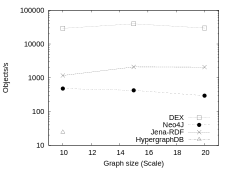
\includegraphics[width=.8\textwidth]{images/benchmarks/ShenResultsInsert}
  \caption{Throughput results from Dominguez-Sal et al.\cite{TaoShen}.}
  \label{fig:throughputShen}
\end{figure}

The research of Dayarathna et al.\cite{Dayarathna2012} used a edge to node ration of 22 with a node count of 1024.
Comparing their results shown in figure~\ref{fig:throughputXGDBench} with our results from figure~\ref{fig:withIndexThroughput} lead to the conclusion,
that the databases perform better with an industrial graph structure and less edges.
The throughput of OrientDB is split in half compared to our workload at the almost same number of nodes (1024 vs. 1000 in our research).
With this observation we come to the conclusion that graph databases would perform even better in an industrial environment,
but since the dataset size which we can compare is too small we cannot surely tell if that holds true for larger node counts.

\begin{figure}[!h]
  \centering
  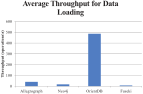
\includegraphics[width=\textwidth]{images/benchmarks/XGDBenchResultsInsert}
  \caption{Throughput results from the XGDBench Benchmark\cite{Dayarathna2012}.}
  \label{fig:throughputXGDBench}
\end{figure}

If we look at our own findings in figure~\ref{fig:indexNoEdges10000Nodes} we can come to the conclusion that the throughput is better when using edges,
which correlates with the comparison to the research conducted by Dominguez-Sal,
but the throughput becomes even better as the number of edges compared to the number of nodes increases and as the ratio of edges to nodes is relatively low in an industrial application that again leads the conclusion,
that graph databases perform worse in the industrial environment and the results of graph benchmarks cannot not be used to determine performance in the industrial internet of things.
